\seite{}{QSS und DEVS}\anchorpage{1}{neu6}{6 · Zustandsquantisierte Simulation und DEVS-Architektur}\ey{KAPITEL 6}\ptitle{Zustandsquantisierte Simulation und DEVS-Architektur}
In einem Heizungsnetz ändern sich einige Speicher rasch, andere halten ihren Wert über Minuten. Weshalb sollte jede Komponente bei jeder kleinen Änderung ihrer Nachbarin neu berechnet werden? Wir lassen jeden Speicher melden, wann sein eigener Zustand einen vorgegebenen Abstand zurückgelegt hat. Nun muss der Rechner den Zeitpunkt aus der Bewegung vorhersagen.
\subt{Der Weg durch das Kapitel}
{\tblstart\begin{tabularx}{\linewidth}{@{}Yr@{}}\toprule
\hyperlink{abs6-1}{6.1 · Quantisierung des Zustands} & \pagelink{abs6-1}\\[2pt]
\hyperlink{abs6-2}{6.2 · QSS1 bis QSS4 und eine globale Fehlerschranke} & \pagelink{abs6-2}\\[2pt]
\hyperlink{abs6-3}{6.3 · Steifigkeit und Chattering bei QSS} & \pagelink{abs6-3}\\[2pt]
\hyperlink{abs6-4}{6.4 · LIQSS und partitionierte Verfahren} & \pagelink{abs6-4}\\[2pt]
\bottomrule\end{tabularx}\par}
\par\vfill{\centering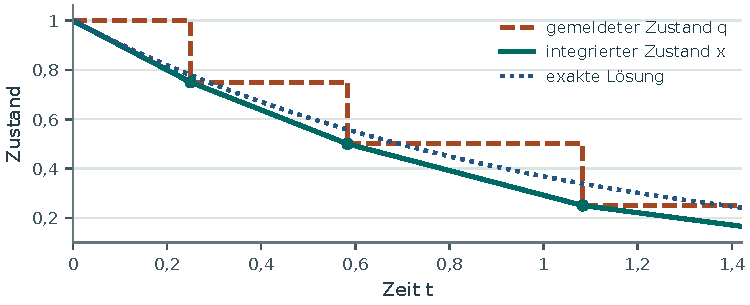
\includegraphics[width=.88\linewidth,height=49mm,keepaspectratio]{qss.pdf}\par}\capline{Die Meldung und der kontinuierliche Zustand haben verschiedene Aufgaben.}
\seite{}{QSS und DEVS}\anchorpage{2}{abs6-1}{6.1 · Quantisierung des Zustands}\ey{ABSCHNITT 6.1}\ptitle{Quantisierung des Zustands}
\hypertarget{punkt6-1-1}{}\subt{6.1.1\enspace Ein Zustand löst eine Meldung aus}
Zeitintegration plant einen Schritt und berechnet den neuen Zustand. QSS führt eine kontinuierliche Näherung \(x\) und ein an das Modell gemeldetes Signal \(q\). Es integriert \(x'=f(q)\) bis zur Grenze des Quantisierungsbandes. Komponenten mit nahezu konstanter Bewegung können lange dieselbe Meldung verwenden. Ob die Implementierung Zeit spart, hängt auch von den Abhängigkeiten und dem Aufwand pro Meldung ab.
\hypertarget{punkt6-1-2}{}\subt{6.1.2\enspace DEVS als Ereignisverwaltung}
Ein atomares DEVS-Modell besitzt Zustand, Ein- und Ausgabe, eine Zeitfortschrittsfunktion sowie interne und externe Übergänge. Der Koordinator wählt das kleinste Fälligkeitsdatum, erstellt die Ausgabe, verteilt Nachrichten und lässt die betroffenen Modelle ihre Termine aktualisieren. Gleichzeitige interne und externe Eingänge benötigen eine festgelegte Konfliktregel. Versionsmarken verhindern, dass ein überholter Eintrag aus der Warteschlange später ausgeführt wird.
\hypertarget{punkt6-1-3}{}\subt{6.1.3\enspace Absolute und relative Quanten}
Für den Speicher in Kelvin sei \(\Delta_i=\max(\Delta_{\min,i},r_i|q_i|)\). Das Band schrumpft beim Abkühlen, der absolute Boden verhindert unendlich kleine Zahlenabstände nahe null. Ein festes Quantum in Metern hat für eine Geschwindigkeit eine andere Bedeutung. Bei einem externen Impuls muss der nächste Termin aus dem neuen Zustand berechnet werden.
\lektion{Wie ein Zustand den nächsten Zeitpunkt bestimmt}{qss}{Kernweg}{Hybride Systeme}
Stellen Sie einer Uhr eine zweite Art von Melder gegenüber. Die Uhr meldet den nächsten vorgegebenen Zeitpunkt. Ein Quantisierer meldet, wann sich eine bestimmte Zustandskomponente um ihr vorgegebenes Quantum geändert hat. Hieraus bauen Quantized-State-System-Verfahren (QSS) eine Integration mit komponentenweise ausgelösten Aktualisierungen. Physikalische Schaltgrenzen kommen bei Bedarf zusätzlich hinzu.
\subt{QSS1 an einem Entladevorgang}
Ein normierter Speicher entlädt sich nach \(y'=-y,\ y(0)=1\). QSS1 integriert \(x'=-q\) und meldet einen konstanten Wert \(q\), bis \(|x-q|=\Delta\) erreicht ist. Beim eigenen Ereignis wird \(q\) auf \(x\) gesetzt. Für \(\Delta=1/4\) gilt zunächst \(x=1-t,\ q=1\). Bei \(t=1/4\) wird \(q=3/4\). Mit der neuen Steigung \(-3/4\) dauert das nächste Viertel im Zustand \(1/3\) Zeiteinheiten. Das zweite Ereignis liegt also bei \(t=7/12\). Die Zeitabstände folgen aus der lokalen Dynamik.
\fig{qss}{.9}{Die gemeldete Treppe bestimmt die Steigung der integrierten Kurve. Die gepunktete Referenz ist \(e^{-t}\). Auch wenn \(x\) und \(q\) nahe beieinanderliegen, ist die Abweichung von der exakten Lösung eine andere Größe.}
\subt{Woher der Ereignismechanismus kommt}
DEVS (\emph{Discrete Event System Specification}) beschreibt einen Baustein mit Zustand, Ein- und Ausgaben, interner und externer Übergangsfunktion, Ausgabefunktion und Zeit bis zum nächsten internen Ereignis. Ein Quantisierer kann so seine nächste Meldung ankündigen. Ändert ein anderer Baustein die Steigung, muss die Vorhersage neu berechnet werden. Für zeitgleiche Ereignisse benötigt das Modell eine eindeutige Regel.
\srcs{\refbk{devs}{Zeigler sowie Zeigler und Lee} · \refbk{qorig}{Kofman und Junco, Quantized-State Systems}.}

\seite{}{QSS und DEVS}\anchorpage{2}{abs6-2}{6.2 · QSS1 bis QSS4 und eine globale Fehlerschranke}\ey{ABSCHNITT 6.2}\ptitle{QSS1 bis QSS4 und eine globale Fehlerschranke}
\hypertarget{punkt6-2-1}{}\subt{6.2.1\enspace QSS1 hält die gemeldete Größe konstant}
Für \(x'=-q\) mit \(x(0)=q(0)=1\) und \(\Delta=0{,}2\) sinkt \(x\) zunächst linear mit Steigung \ensuremath{-}1. Die erste Meldung erfolgt nach 0,2 Zeiteinheiten bei \(x=0{,}8\). Die zweite Flugzeit beträgt \(0{,}2/0{,}8=0{,}25\). Der kontinuierliche Zustand bewegt sich auch zwischen den Meldungen.
\hypertarget{punkt6-2-2}{}\subt{6.2.2\enspace Polynome und die nächste positive Wurzel}
QSS2 meldet eine Gerade, QSS3 ein quadratisches und QSS4 ein kubisches Polynom. Der integrierte Zustand hat im idealen Taylor-Verfahren jeweils einen Grad mehr. Man bildet \(x_i(s)-q_i(s)\mp\Delta_i\), sucht die kleinste zulässige positive Wurzel und prüft die Richtung. Eine Wurzel nahe null unmittelbar nach einer Meldung braucht eine eigene Behandlung. Der konkrete QSS2-Termin steht auf S.\,\pagelink{qzahl}.
\hypertarget{punkt6-2-3}{}\subt{6.2.3\enspace Beweis am stabilen linearen Speicher}
Sei \(y'=-ay+u,\ x'=-aq+u,\ a>0\) und überall \(|q-x|\le\Delta\). Mit \(e=x-y\) folgt \(e'=-ae-a(q-x)\). Multiplikation mit \(e^{at}\) und Integration liefert
\[
 |e(t)|\le e^{-at}|e(0)|+a\Delta\int_0^te^{-a(t-s)}\,ds
 = e^{-at}|e(0)|+(1-e^{-at})\Delta .
\]
Die Schranke gilt für alle Zeiten des glatten Abschnitts. Sie beschreibt die gedämpfte Fehlerantwort. Zusätzliche numerische Ableitungs- und Resetfehler müssen separat eingehen.
\notebox{Merksatz}{Für einen stabilen linearen Vektorspeicher mit \(\|e^{At}\|\le M e^{-\gamma t}\), \(\gamma>0\), gilt bei \(\|q-x\|\le\Delta\) und \(e=x-y\) die Gleichung \(e'=Ae+A(q-x)\). Variation der Konstanten und Integration von \(e^{-\gamma(t-s)}\) ergeben \(\|e(t)\|\le M e^{-\gamma t}\|e(0)\|+M\|A\|\Delta(1-e^{-\gamma t})/\gamma\). Für gekoppelte Speicher kann der Verstärkungsfaktor größer als eins sein.}
\lektion{Wie der Quantisierungsfehler die Lösung stört}{qfehler}{Vertiefung}{Hybride Systeme}
Die diskrete Meldung \(q\) verändert die rechte Seite. Das Quantum hat die Einheit des zugehörigen Zustands. Ein Quantum von einem Millimeter bei der Position und eines von einem Ampere beim Strom sind ohne getrennte Skalierung unvergleichbar.
\subt{Satz · Fehlergrenze für einen stabilen skalaren Speicher}
Es gelte \(y'=-ay,\ x'=-aq,\ a>0,\ x(0)=y(0)\) und während des gesamten Versuchs \(|x-q|\le\Delta\). Dann gilt
\[
 |x(t)-y(t)|\le\Delta(1-e^{-at}).
\]
\proofpart{Mit \(e=x-y,\ \delta=x-q\) ergibt sich \(e'=-ae+a\delta\). Variation der Konstanten liefert \(e(t)=a\int_0^t e^{-a(t-s)}\delta(s)\dg s\). Der Betrag ist höchstens \(a\Delta\int_0^t e^{-a(t-s)}\dg s\). Auswerten des Integrals ergibt die Behauptung.}
Die Abschätzung nutzt die dämpfende skalare Gleichung. In gekoppelten Systemen wirkt ein Quantisierungsfehler über die Dynamik auf andere Komponenten. Ein kleines Quantum allein garantiert keine bestimmte Stoßzeit. Liegt ein Wächter fast tangential zur Bahn, kann schon eine kleine Zustandsabweichung die geschätzte Zeit stark verschieben.
\subt{Ein äußerer Eingang widerruft einen Termin}
Für \(x'=u\), \(x(0)=q(0)=0\), \(\Delta=1/4\), \(u=1\) ist die erste Meldung bei \(t=1/4\) vorgesehen. Bereits bei \(t=1/8\) springt der Eingang auf \(-1\). Dann steht \(x=1/8,\ q=0\). Die neue Grenze liegt bei \(-1/4\), also noch \(3/8\) Zeiteinheiten entfernt. Der nächste Meldetermin ist \(t=1/2\). Eine unverändert ausgelöste Meldung beim alten Termin wäre ein Fehler in der Ablaufsteuerung.
\notebox{Lokale Arbeit}{Ein Zustandsereignis verändert nur jene rechten Seiten, die den gemeldeten Zustand tatsächlich verwenden. Ein dünn besetzter Abhängigkeitsgraph spart Arbeit, wenn der Simulator lokale Aktualisierungen umsetzt und die Komponenten zu unterschiedlichen Zeiten aktiv sind. Der Python-Referenzcode im Projekt verwendet auch dichte Auswertungen.}
\srcs{\refbk{qorig}{QSS-Grundlage} · \refbk{qrev}{Übersicht zu QSS} · \repo{docs/SOLVER_SELECTION.md}{Implementierung und Kosten}.}

\lektion{Vom Quantum zur nächsten Meldung}{qzahl}{Rechenversuch}{Nachweise zum Modell}
\subt{QSS2 · Ein Fehlerpolynom von Hand auswerten}
Für \(x'=-q,\ x(0)=1\) meldet QSS2 anfangs Wert und Steigung, also \(q(t)=1-t\). Integration liefert \(x(t)=1-t+t^2/2\). Bei \(\Delta=0{,}02\) erreicht \(|x-q|=t^2/2\) erstmals im Zeitpunkt \(t=0{,}2\) das Quantum. Direkt davor gelten \(x=0{,}82\) und \(q=0{,}8\). QSS3 benutzt analog eine quadratische Meldung und eine kubische Bahn, bei der QSS4-Erweiterung steigen beide Grade um eins.
\subt{Drei Regeln am stabilen Speicher}
Für \(x'=-q\) und \(x(0)=100\) frieren wir die Meldung jeweils bis zum ersten Termin ein oder wählen vorab ihren Zielwert:
\begin{itemize}\zerolist
\item Relatives QSS1 meldet zunächst \(q=100\). Mit \(\max(0{,}01;0{,}1|x|)=10\) wird nach \(0{,}1\) bei \(x=90\) neu gemeldet. Dann beträgt das Quantum 9.
\item CQSS1 mit Zellbreite 10 meldet anfangs den Mittelpunkt 100. Die untere Fläche liegt bei 95. Sie wird nach \(0{,}05\) erreicht, dann meldet die folgende Zelle ihren Mittelpunkt 90.
\item BQSS1 prüft vor der Integration die Richtung und wählt für Quantum 10 das vorausliegende Ziel 90. Damit gilt \(x'=-90\), und das Ziel wird nach \(1/9\) erreicht. Zeigt die dort ausgewertete Steigung in einem gekoppelten Versuch weg vom Ziel, hält die Implementierung die Komponente bis zur nächsten möglichen Änderung an.
\end{itemize}
\srcs{\see{qkatalog}{Verfahrensübersicht} · \repocurrent{argesim_benchmarks/solvers/backward_qss.py}{Zielwahl und Halteregel}.}

\seite{}{QSS und DEVS}\anchorpage{2}{abs6-3}{6.3 · Steifigkeit und Chattering bei QSS}\ey{ABSCHNITT 6.3}\ptitle{Steifigkeit und Chattering bei QSS}
\hypertarget{punkt6-3-1}{}\subt{6.3.1\enspace Wenn ein schnelles Rückstellglied zu viele Meldungen erzeugt}
Liegt das Gleichgewicht einer stark gedämpften Komponente mitten im Band, kann die eingefrorene Steigung den Zustand darüber hinaustragen. Beim Melden wechselt das Vorzeichen. Der Speicher pendelt numerisch, obwohl das physikalische System rasch in Ruhe käme. Ein typischer Diagnoseversuch zeichnet \(x_i,q_i\) und die Meldedichte zusammen auf und verkleinert dann das Quantum. Numerische Meldungen und physikalische Schaltungen sind getrennte Zähler.

Rechnen Sie einen solchen Umlauf selbst. Für \(x'=-a q\), \(a>0\), verwendet QSS1 die Aktualisierung \(q\leftarrow x\), sobald \(|x-q|=\Delta\). Starten wir mit \(q=x=\Delta/2\). Die Steigung beträgt \(-a\Delta/2\). Um bis \(-\Delta/2\) zu reisen, muss \(x\) die Strecke \(\Delta\) zurücklegen. Das dauert \(\Delta/(a\Delta/2)=2/a\). Jetzt kehrt die Steigung ihr Vorzeichen um. Nach weiteren \(2/a\) ist der Ausgangswert wieder erreicht. Bei diesem gewählten Start halbiert ein halb so großes Band samt halbiertem Startwert die Schwingungsamplitude. Die Periodendauer \(4/a\) bleibt gleich. Die exakte Lösung \((\Delta/2)e^{-at}\) fällt dagegen fortlaufend.
\seite{}{QSS und DEVS}\anchorpage{2}{abs6-4}{6.4 · LIQSS und partitionierte Verfahren}\ey{ABSCHNITT 6.4}\ptitle{LIQSS und partitionierte Verfahren}
\hypertarget{punkt6-4-1}{}\subt{6.4.1\enspace Lokale implizite Rückkopplung}
LIQSS nähert die eigene Abhängigkeit als \(x_i'\simeq a_{ii}x_i+u_i\) an. Im Dämpfungsfall \(a_{ii}<0\) gibt \(-u_i/a_{ii}\) das lokale Gleichgewicht an. Die Quantisierungsentscheidung berücksichtigt es und kann die unphysikalische Banddurchquerung vermeiden. Bei zwei stark rückgekoppelten Zuständen enthält die Diagonale nur einen Teil der Dynamik. Eine Paarbehandlung oder ein Blocksolve kann angemessener sein.
\hypertarget{punkt6-4-2}{}\subt{6.4.2\enspace eLIQSS und die Bandbreite}
Erweiterte Quantisierer wählen das Startpolynom so, dass seine Differenz zum fortgeführten Zustand einen größeren zulässigen Teil des Bandes ausnutzt. Die erwartete Flugzeit wird unter den örtlichen Modellannahmen verlängert. Eine externe Nachricht kann jede Prognose vorzeitig beenden. Im Projekt ergeben eLIQSS1 und CheQSS1 dieselbe mathematische Aktualisierung.
\hypertarget{punkt6-4-3}{}\subt{6.4.3\enspace LIQSS–BDF über eine Blockgrenze}
In der Projektvariante übernimmt LIQSS2 die quantisierten Komponenten, BDF1/2 den angegebenen steifen Block. An der gemeinsamen Zeit müssen beide Blöcke mit verträglichen Kopplungswerten rechnen. Scheitert die Kopplungsiteration, darf kein Teilzustand vorzeitig festgeschrieben werden. Für den Vergleich zählen auch diese Iterationen, Neuplanungen und verworfenen Versuche.
\srcs{\repocurrent{docs/SOLVER_METHODS.md}{Quantisierer im Projekt} · \refbk{qorig}{Literatur zur Zustandsquantisierung}.}
\lektion{Die quantisierten Methoden im Vergleich}{qkatalog}{Vertiefung}{Hybride Systeme}
Die Ordnungszahl beschreibt die Konstruktion auf glatten Abschnitten. Bei explizitem QSS der Ordnung \(p\) hat der gemeldete Verlauf typischerweise Grad \(p-1\) und der integrierte Verlauf Grad \(p\). QSS2 kann damit eine freie Bewegung mit konstanter Geschwindigkeit auf dem jeweiligen Abschnitt darstellen. Ein physikalischer Kontakt muss weiterhin lokalisiert werden.
{\tblstart\begin{tabularx}{\linewidth}{@{}P{28mm}Y@{}}\toprule
\hd{Familie}&\hd{Rechenidee und geeigneter Versuch}\\\midrule
QSS1 bis QSS4&Konstante, lineare, quadratische oder kubische Meldung. Höhere Ordnung lohnt auf glatten Abschnitten, sofern zusätzliche Ableitungsarbeit und Nullstellensuche sich auszahlen.\\
CQSS1&Zentrierte Zelle ohne Hysterese. Für geeignete geometrische Systeme interessant. An Zellgrenzen können unmittelbare Rückwechsel den Zeitfortschritt verhindern.\\
LIQSS1 bis 3&Lokale lineare Selbstkopplung über den Diagonaleintrag der Jacobi-Matrix. Eine schnelle Komponente kann einem nahen Gleichgewicht folgen.\\
mLIQSS1 bis 3&Stark rückgekoppelte Paare werden gemeinsam behandelt. Das erhöht den Aufwand je Meldung. Die Variante dritter Ordnung ist eine experimentelle Projekterweiterung.\\
eLIQSS1 bis 3&Nutzt den vom Fehlerpolynom erlaubten Teil des Quantisierungsbands bis zum nächsten geplanten Ereignis.\\
CheQSS1 bis 3&Verteilt den Fehler mit verschobenen Tschebyscheff-Polynomen. In erster Ordnung ist die Aktualisierung dieselbe wie bei eLIQSS1.\\
LIQSS-BDF&Teilt Zustände in eine quantisierte und eine implizit zeitintegrierte Gruppe. Auf der BDF-Seite dienen rückwärts Euler und BDF2 als Schritte. Partition und Austausch müssen zur Kopplung passen.\\\bottomrule
\end{tabularx}\par}
Die Acht-Fälle-Matrix enthält damit 18 registrierte QSS-Namen. Die spätere Auswahlstudie ergänzt BQSS1, das vorwärts liegende Gitterwerte anhand der Bewegungsrichtung auswählt, sowie QSS1/2 mit logarithmischer Quantisierung. Dabei wird die Breite bei einem eigenen Update aus \(\max(\Delta_\mathrm{abs},\Delta_\mathrm{rel}|x_i|)\) bestimmt. Relative Quanten helfen bei großen Dynamikbereichen. Die absolute Untergrenze ist nahe null entscheidend.
\srcs{\repo{QSS_SOLVERS.md}{Methodenkatalog des Projekts} · \refbk{liq}{Migoni u.\,a., LIQSS} · \see{matrix}{alle 18 Namen und ihre Trefferzahlen} · \see{qzahl}{Drei Quantenregeln und der erste QSS2-Termin}.}
\lektion{Zwei Quantisierer melden gleichzeitig}{pruefung6}{Herleitung und Gegenprobe}{Kapitel 6}
Zwei Speicher werden mit der gleichen konstanten Rate geladen. Beide melden nach \(0{,}2\unitm s\) einen Banddurchgang. Ein dritter Baustein erhält die Differenz \(q_1-q_2\). In der richtigen Trajektorie ist diese Differenz null. Wenn das Programm die erste Meldung schon wirksam macht und erst später die zweite einsammelt, erzeugt es eine künstliche Zwischenstufe. Wie legt man fest, was „gleichzeitig“ im Rechner bedeutet?

Für diesen Lehrversuch sei \(x'_1=x'_2=1\), \(x'_3=q_1-q_2\) und \(x(0)=q(0)=0\) bei einheitlich skalierten Zuständen. QSS1 hält \(q_1,q_2\) zwischen ihren Meldungen konstant. Das Quantum sei jeweils \(0{,}2\). Bei \(t=0{,}2\) sind die kontinuierlichen Zustände \(x_1=x_2=0{,}2\). Beide quantisierten Ausgänge wechseln im gleichen Ereigniszeitpunkt auf \(0{,}2\). Für das anschließende offene Zeitintervall ist also \(x'_3=0\). Bei \(t=0{,}4\) wiederholt sich die Rechnung. Wer nach der ersten Meldung \(x'_3=0{,}2\) findet, muss beim zweiten Eingang am gleichen Zeitpunkt die Prognose erneut bilden. Für das Fortschreiben von \(x_3\) ist dabei null physikalische Zeit vergangen.

Der Koordinator sammelt alle für denselben Termin gültigen internen Ausgaben aus dem alten Zustand, verteilt sie als Eingabemenge und führt erst dann die Zustandsübergänge aus. Treffen interne und externe Termine eines Bausteins zusammen, legt seine konfluente Übergangsfunktion die gemeinsame Verarbeitung fest. Zeitstempel mit einem zusätzlichen Mikroindex ordnen Folgereaktionen bei derselben physikalischen Zeit.
\notebox{Achtung, Falle}{Das willkürliche Zusammenziehen numerisch naher, tatsächlich verschiedener Zeiten kann die Ereignisfolge ändern. Im Versuch lassen sich die gemeinsamen Termine über denselben ganzzahligen Taktindex erzeugen. Prüfen Sie die dritte Trajektorie noch einmal bei umgekehrter Einfügereihenfolge der Meldungen.}
\srcs{\see{alg6}{Veraltete Termine im Kalender} · \see{qfehler}{Vom Quantenband zur globalen Fehlerschranke}.}

\lektion{Eine überholte QSS-Meldung erkennen}{alg6}{Werkstatt}{Kapitel 6}
Eine alte Prognose kann beim Eintreffen einer Nachricht noch in der Prioritätswarteschlange liegen. Verwaltet jeder Speicher eine fortlaufende Versionsnummer, erkennt der Koordinator veraltete Einträge, bevor sie den Zustand verändern.
{\small\begin{verbatim}
(t, i, version) = fruehester_Eintrag()
wenn version != aktuell[i]: ueberspringe_Eintrag
sammle_alle_gueltigen_Meldungen_zur_selben_Zeit(t)
fuehre_Polynome_bis(t)
sende interne Ausgaben aus den Zustaenden vor dem Wechsel
sammle fuer jedes Modell alle eintreffenden Eingaben
intern und extern: verwende die konfluente Modellregel
sonst: verwende den internen oder externen Uebergang
fuer jede betroffene Komponente j:
    aktuell[j] += 1
    plane(neuen_Banddurchgang(j), j, aktuell[j])
\end{verbatim}}
\subt{Selbst rechnen}
Ein Speicher erwartet den nächsten Durchgang bei 0,45 s. Um 0,3 s setzt eine externe Nachricht seine Steigung auf null. Wann darf der alte Durchgang den Zustand verändern?
\notebox{Lösung}{Mit der neuen Version ist der Termin bei 0,45 s ungültig. Bleibt der Zustand strikt im Band und die Steigung null, ist die nächste interne Zeit unendlich. Erst eine weitere Eingabe kann einen neuen endlichen Termin erzeugen.}
